\documentclass[conference]{IEEEtran}
\IEEEoverridecommandlockouts
% The preceding line is only needed to identify funding in the first footnote. If that is unneeded, please comment it out.
\usepackage{cite}
\usepackage{amsmath,amssymb,amsfonts}
\usepackage{graphicx}
\usepackage{textcomp}
\usepackage{xcolor}
\usepackage{url}
\usepackage{enumerate}
\usepackage{makecell}
\usepackage{listings}
\usepackage{wrapfig}
\usepackage{paralist}
\usepackage{xspace}
\usepackage{color}
\usepackage{times}
\usepackage{proof}
\usepackage{algorithm}
\usepackage[noend]{algpseudocode}
\usepackage{capt-of}

%%


%Transition system
\newcommand{\TS}[1]{\ensuremath{\mathcal{T}_{#1}}}
\newcommand{\states}[1]{\ensuremath{\mathcal{C}_{#1}}}
\newcommand{\transitions}[1]{\ensuremath{\mathcal{R}_{#1}}}
\newcommand{\transition}[1]{\ensuremath{\mathit{t}_{#1}}}
\newcommand{\labels}[1]{\ensuremath{\Sigma_{#1}}}
\newcommand{\enable}[1]{\ensuremath{\mathit{en}_{#1}}}
\newcommand{\reachstates}[1]{\ensuremath{\mathit{RS}_{#1}}}

\newcommand{\location}[1]{\ensuremath{\mathit{L}_{#1}}}
\newcommand{\regionstructure}[1]{\ensuremath{\mathcal{S}_{#1}}}
\newcommand{\regions}[1]{\ensuremath{\mathcal{Q}_{#1}}}

%\newcommand{\AP}{\mathit{AP}}

\newcommand{\reaches}{\ensuremath{\leadsto}}

% BIP
\newcommand{\BIP}{\ensuremath{\textsc{BIP}}\xspace}
\newcommand{\bipvar}[1]{\ensuremath{\mathbb{V}_{#1}}}
\newcommand{\varstate}[1]{\ensuremath{\mathbf{V}_{#1}}}
\newcommand{\locs}[1]{\ensuremath{\mathbb{L}_{#1}}}
\newcommand{\locerr}[1]{\ensuremath{\mathbb{L}_{err_{#1}}}}
\newcommand{\ports}[1]{\ensuremath{\mathbb{P}_{#1}}}
\newcommand{\edges}[1]{\ensuremath{\mathbb{E}_{#1}}}
\newcommand{\init}[1]{\ensuremath{\mathbb{I}_{#1}}}
\newcommand{\allports}{\ensuremath{\bigcup_{i = 1}^n{\ports{i}}}}
\newcommand{\bexp}[1]{\ensuremath{\mathcal{F}_{#1}}}
\newcommand{\expr}[1]{\ensuremath{\mathcal{E}_{#1}}}
\newcommand{\compstate}[1]{\ensuremath{\langle l_{#1}, \mathbf{V}_{#1} \rangle}}
\newcommand{\components}{\ensuremath{\mathcal{B}}}
\newcommand{\bipmodel}{\ensuremath{\mathcal{M}_{\BIP}}}
\newcommand{\comp}[1]{\ensuremath{B_{#1}}}
\newcommand{\region}[1]{\ensuremath{\langle l_{#1}, \phi_{#1} \rangle }}
\newcommand{\portid}[1]{{\ensuremath{id({#1})}}}

\newcommand{\variable}[1]{\ensuremath{\mathbb{V}_{#1}}}



%ART
%\newcommand{\region}[1]{\ensuremath{\psi_{#1}}}
\newcommand{\ART}[1]{\ensuremath{\mathbb{T}_{#1}}}
\newcommand{\artnode}[1]{\ensuremath{\mathit{nd}_{#1}}}
\newcommand{\artroot}{\ensuremath{\mathit{Root}}}
\newcommand{\nodes}{\ensuremath{\mathit{Nodes}}}
\newcommand{\artedge}{\ensuremath{\mathit{Edges}}}
\newcommand{\covers}{\ensuremath{\mathit{Covers}}}
\newcommand{\artpath}{\ensuremath{\pi}}
\newcommand{\interpolant}[1]{\ensuremath{\mathbf{I}_{#1}}}
\newcommand{\cex}[1]{\ensuremath{\mathit{cex}_{#1}}}
\newcommand{\leafs}{\ensuremath{\mathit{Leafs}}}


% POR
\newcommand{\enabled}{\ensuremath{\Gamma_{enab}}}
\newcommand{\sset}{\ensuremath{\Gamma_{sim}}}
\newcommand{\pset}{\ensuremath{\Gamma_{per}}}
\newcommand{\aset}{\ensuremath{\Gamma_{amp}}}
\newcommand{\sbset}{\ensuremath{\Gamma_{stub}}}

%
% Useful symbols and abbreviations
%
\newcommand{\Nat}{\mathbb{N}}    % natural numbers
\newcommand{\Real}{\mathbb{R}}   % real numbers
\newcommand{\Int}{\mathbb{Z}}    % integers
\newcommand{\xone}[2]{#1_1,\ldots,#1_{#2}}   % variable range from 1
\newcommand{\xzero}[2]{#1_0,\ldots,#1_{#2}}  % variable range from 0
\newcommand{\CalC}{\mathcal{C}}              % example of caliph C
\newcommand{\setof}[1]{\{#1\}}               % set
\newcommand{\powerset}[1]{2^{#1}}   % power set
\newcommand{\Def}{\stackrel{\mathrm{def}}{=}}   % definition
\newcommand{\mktuple}[1]{\ensuremath{\langle{#1}\rangle}} % tuple definition
\newcommand{\true}{\ensuremath{\mathit{true}}}
\newcommand{\false}{\ensuremath{\mathit{false}}}


% Software model checkers and tools.
\newcommand{\kratos}{\textsc{Kratos}\xspace}
\newcommand{\nusmv}{\textsc{NuSMV}\xspace}
\newcommand{\nuxmv}{\textsc{nuXmv}\xspace}
\newcommand{\mathsat}{\textsc{MathSAT}\xspace}
\newcommand{\dfinder}{\textsc{DFinder}\xspace}
\newcommand{\vcs}{\textsc{VCS}\xspace}


\newtheorem{definition}{Definition}

\def\BibTeX{{\rm B\kern-.05em{\sc i\kern-.025em b}\kern-.08em
    T\kern-.1667em\lower.7ex\hbox{E}\kern-.125emX}}
\begin{document}

\title{Behavioral fault modeling and analysis with SBIP:
	A Wheel Brake System Case Study\\}

\author{\IEEEauthorblockN{1\textsuperscript{st} Xudong Tang}
\IEEEauthorblockA{\textit{Shanghai Key Lab for Trustworthy Computing} \\
\textit{East China Normal University }\\
Shanghai, China \\
51184501045@stu.ecnu.edu.cn}
\and
\IEEEauthorblockN{2\textsuperscript{nd} Qiang Wang}
\IEEEauthorblockA{\textit{dept. name of organization (of Aff.)} \\
\textit{name of organization (of Aff.)}\\
City, Country \\
email address or ORCID}
\and
\IEEEauthorblockN{3\textsuperscript{rd} Weikai Miao}
\IEEEauthorblockA{\textit{dept. name of organization (of Aff.)} \\
\textit{name of organization (of Aff.)}\\
Shanghai, China \\
wkmiao@sei.ecnu.edu.cn}
}

\maketitle

\begin{abstract}
Behavior-Interaction-Priority(BIP) is a component-based framework for modeling complex systems. According to BIP framework, system can be represented by a set of components specifying the behavior which is synchronized and communicated by connectors that corresponds to subset of interactions.
Behavioral fault modeling and analysis refers to an integration of model based system design and safety analysis. In this paper, we integrate fault-tree-based safety analysis into BIP model and using statistical model checking engine for the BIP framework(SBIP) to offer a stochastic information to components and the entire system. By using SBIP with statistic model checking, we verify system specification and calculate probability of fault issues. We also trace the simulation result to confirm the extended system model without fault keeps consistence of the norminal system model.  
We illustrate an airplane wheel brake system meeting the industry standards as case study to show its advantage in analyzing fault behavior of safety-critical systems in aerospace practice.
\end{abstract}

\begin{IEEEkeywords}
model checking, safety analysis, fault tree, BIP
\end{IEEEkeywords}

\section{Introduction}
Giving introduction of BIP framework, BIP toolset, SBIP and, on the other hand, faulttree-based safety analysis. Using structure of the paper as ending.

\section{Preliminaries}

\subsection{The BIP Framework}
We use architecture diagrams \cite{} to model the architecture styles in BIP.
An architecture diagram consists of a set of component types, with associated cardinality constraints representing the
expected number of instances of each component type and a set of connector motifs.
Connector motifs, which define sets of BIP connectors, are non-empty sets of port types, each labelled as either a trigger or a synchron.
Each port type has a cardinality constraint representing the expected number of port instances
per component instance and two additional constraints: multiplicity and degree,
represented as a pair m : d. Multiplicity constrains the number of instances of
the port type that must participate in a connector defined by the motif; degree
constrains the number of connectors attached to any instance of the port type.

In this section, we present the BIP model with multiparty synchronization and data transfer.A BIP model is a parallel composition of a set of components.
A BIP component is formally defined as an automaton extended with linear integer arithmetic as follows.

\begin{definition} [BIP component]
	\label{component-def}
	Given a finite set of variables $\bipvar{}$, a BIP component is defined as a tuple
	$\comp{} = \mktuple{\bipvar{}, \locs{}, \ports{}, \edges{}, \ell}$, where
	\begin{inparaenum}
		\item $\locs{}$ is a finite set of control locations;
		\item $\ports{}$ is a finite set of communication ports;
		\item $\edges{} \subseteq \locs{} \times \ports{} \times \bexp{\bipvar{}} \times \expr{\bipvar{}} \times \locs{}$
		is a finite set of transition edges extended with guards in $\bexp{\bipvar{}}$
		and operations in $\expr{\bipvar{}}$;
		\item $\ell \in \locs{}$ is an initial control location.
	\end{inparaenum}
\end{definition}

Transition edges in a component are labeled by ports, which form the interface of the component.
We assume that, from each control location,
every pair of outgoing transitions have different ports,
and the ports of different components are disjoint.
In other words, transitions with the same ports in the component are not enabled simultaneously.
Given a component violating such assumptions,
one can easily transform it into the required form by renaming the ports,
while retaining the BIP expressiveness power.
To ease the presentation, we denote in the sequel the id of the unique component
where port $p$ is defined by $\portid{p}$.

%Given a tuple of component types $\overline{\comptype{}} = \mktuple{\comptype{1},\ldots, \comptype{k}}$,
%and a tuple of natural numbers $\overline{n} = \mktuple{n_{1}, \ldots, n_{k}}$,
%where $n_{i}$ represents the number of instantiations of $\comptype{i}$,
%

We denote by $\components = \{\comp{i} ~|~ i\in [1,n]\}$ a set of components.
%instantiated from $\overline{\comptype{}}$.
%where $\comptype{i}[j]$
%$\comptype{i}[j] = \mktuple{\bipvar{i}[j] ,\locs{i}[j] ,\ports{i}[j], \edges{i}[j], \ell_{i}[j] }$
%is the $j^{th}$ instantiation of component type $\comptype{i}$.
%
%Given a set of comoponents $\components$,
In \BIP, coordinations of components are specified by using interactions.
%and in \BIP an interaction is represented as a finite set of ports.

\begin{definition} [Interaction]
	\label{interaction}
	An interaction for $\components $ is a tuple $\gamma = \mktuple{g, \mathcal{P}, f } $,
	where $g \in \bexp{\bipvar{}}$, $f\in \expr{\bipvar{}}$ and
	$\mathcal{P} \subseteq \bigcup_{i=1}^n \ports{i}$, $\mathcal{P} \neq \emptyset$, and
	for all $i \in [1, n]$, $|\mathcal{P} \cap \ports{i}| \le 1$.
\end{definition}

Intuitively, an interaction defines a guarded multiparty synchronization with data transfer:
when the guard $g$ of an interaction $\mathcal{P}$ is enabled,
then the data transfer specified by $f$ can be executed, and
after that the transitions labelled by the ports in $\gamma$ can be taken simultaneously.
%
We denote by $\Gamma$ a finite set of interactions.
A \BIP model is constructed by composing a number of components with interactions.

\begin{definition} [\BIP Model]
	A \BIP model $\bipmodel$ is a tuple $\mktuple{\components,\Gamma}$,
	where $\components$ is a finite set of components,
	and $\Gamma$ is a finite set of interactions for $\components$.
\end{definition}

We do not take priority into account in this paper, as in the previous work~\cite{dfinder10,tgc15},
since adding priority will not introduce any errors.
If a model without priority is safe, then after adding priority constraints it remains safe.
We use a simple mutual exclusion protocol to illustrate \BIP.

%\input{ticket-bip}

A state of a \BIP model is a tuple $c = \langle \compstate{1}, \ldots, \compstate{n} \rangle $,
where for all $i \in [1,n] $, $l_i \in \locs{i} $ and $\mathbf{V}_i $ is a valuation of $\bipvar{i}$.
%
%We denote by $c(i,j), i\in[1,k]$ the state $\mktuple{l_{i}^{j}, s_{i}^{j}}$ of component $\comptype{i}[j]$.
%$c_0=\mktuple{\mktuple{l_1,s_1},\ldots, \ldots, \mktuple{l_n,s_n}}$
A state $c_{0}$ is initial if for all $i \in [1,n]$,
$l_i = \ell_{i}$ and $\mathbf{V}_{i}$ is the initial valuation of $\bipvar{i}$.
%
A state $c$ is an error if for some $i \in [1,n]$, $l_{i}$ is an error location.
%
We say an interaction $\gamma \in \Gamma$ is enabled on a state $c$ if
for every component $\comp{i} \in \components$,
such that $\gamma \cap \ports{i} \neq \emptyset$,
%
there is an edge $\mktuple{l_i, \gamma \cap \ports{i}, g_i, f_i, l_{i}' } \in \edges{i}$
and  $\mathbf{V}_{i} \models g_i $.
%
The labeled transition system semantics of a \BIP model is defined as follows.

\begin{definition} [\BIP operational semantics]
	\label{operational-semantics}
	Given a \BIP model $\bipmodel=\mktuple{\components,\Gamma}$,
	its operational semantics is defined by a labeled transition system
	$\TS{\BIP} = \mktuple{\mathcal{C}, \Sigma, \mathcal{R}, \mathcal{C}_{0}}$, where
	%
	\begin{enumerate}
		\item $\mathcal{C}$ is the set of states,
		\item $\Sigma = \Gamma $,
		\item $\mathcal{R}$ is the set of transitions,
		and we say that there is a transition from a state $c$
		%$c=\mktuple{\mktuple{l_1,s_1}, \ldots, \mktuple{l_n,s_n}} $
		to another state $c'$,
		%$c'=\mktuple{\mktuple{l_1',s_1'}, \ldots, \mktuple{l_n',s_n'}}$
		if there is an interaction $\gamma $ such that,
		%
		\begin{enumerate}
			%\begin{inparaenum}[(i)]
			\item $\gamma$ is enabled in $c$;
			\item for all $\comp{i} \in \mathbb{B}$ such that
			$\gamma \cap \ports{i} \neq \emptyset$, there is an edge
			$\mktuple{l_i, \gamma \cap \ports{i}, g_i, f_i, l_i'} \in \edges{i} $,
			%and if $f_i = x := e $,
			then $\mathbf{V}'_{i} = \mathbf{V}_{i}[\bipvar{} / f_i(\bipvar{})]$;
			\item for all $\comp{i} \in \mathbb{B} $ such that
			$\gamma \cap \ports{i} = \emptyset $,
			$l_i' = l_i$ and $\mathbf{V}_i' = \mathbf{V}_i$.
			%\end{inparaenum}
		\end{enumerate}
		\item $\mathcal{C}_{0}$ is the set of initial states.
	\end{enumerate}
\end{definition}

%We denote by $c \overset{\gamma} \rightarrow c'$ that
%there is a transition from state $c$ to state $c'$, following the interaction $\gamma$.
%
%We denote by $\rho$
%
%A state $c$ % $c=\mktuple{\mktuple{l_1,s_1}, \ldots, \mktuple{l_n,s_n}}$
%is reachable if there is a trace
%$c_0, c_1, \ldots, c_k$ such that
%$c_0 \xrightarrow{\gamma_1} c_1 \xrightarrow{\gamma_2} \ldots \xrightarrow{\gamma_k} c $,
%from an initial configuration $c_{0}$ to $ c$.
%
In this paper, we do not use temporal logics to specify safety properties,
but recognize a set of locations as error locations.
A \BIP model is safe if no error states are reachable.
Notice that any safety property can be encoded as a reachability
problem by necessarily creating additional components.

\subsection{Statistical Model Checking}
Giving an introduction of Statistical Model Checking here.

\section{The AIR6110 Wheel Brake System}
The Wheel Brake System(WBS) description is introducted in Aerospace Information Report 6110(AIR6110)[] as a contiguous aircraft system development process example. According to AIR6110 standard, WBS is a detailed funciton of an aircraft designated model S18. The hypothetical S18 aircraft is a two engine passenger aircraft designed to carry 300 to 350 passengers up to 5000 nautical miles at
0.84 mach, and has an average flight duration of 5 hours. The WBS provides braking on the main gear wheels used to provide safe retardation of the aircraft during taxiing and landing phases, and in the event of a rejected take-off. The wheel brakes also prevent unintended aircraft motion when parked, and may be used to provide differential braking for aircraft directional control. A secondary function of the WBS is to stop main gear wheel rotation upon gear retraction. Braking on the ground is commanded manually, via brake pedals, or automatically (autobrake) without the need for pedal application.

\begin{figure}[htbp]
	\centerline{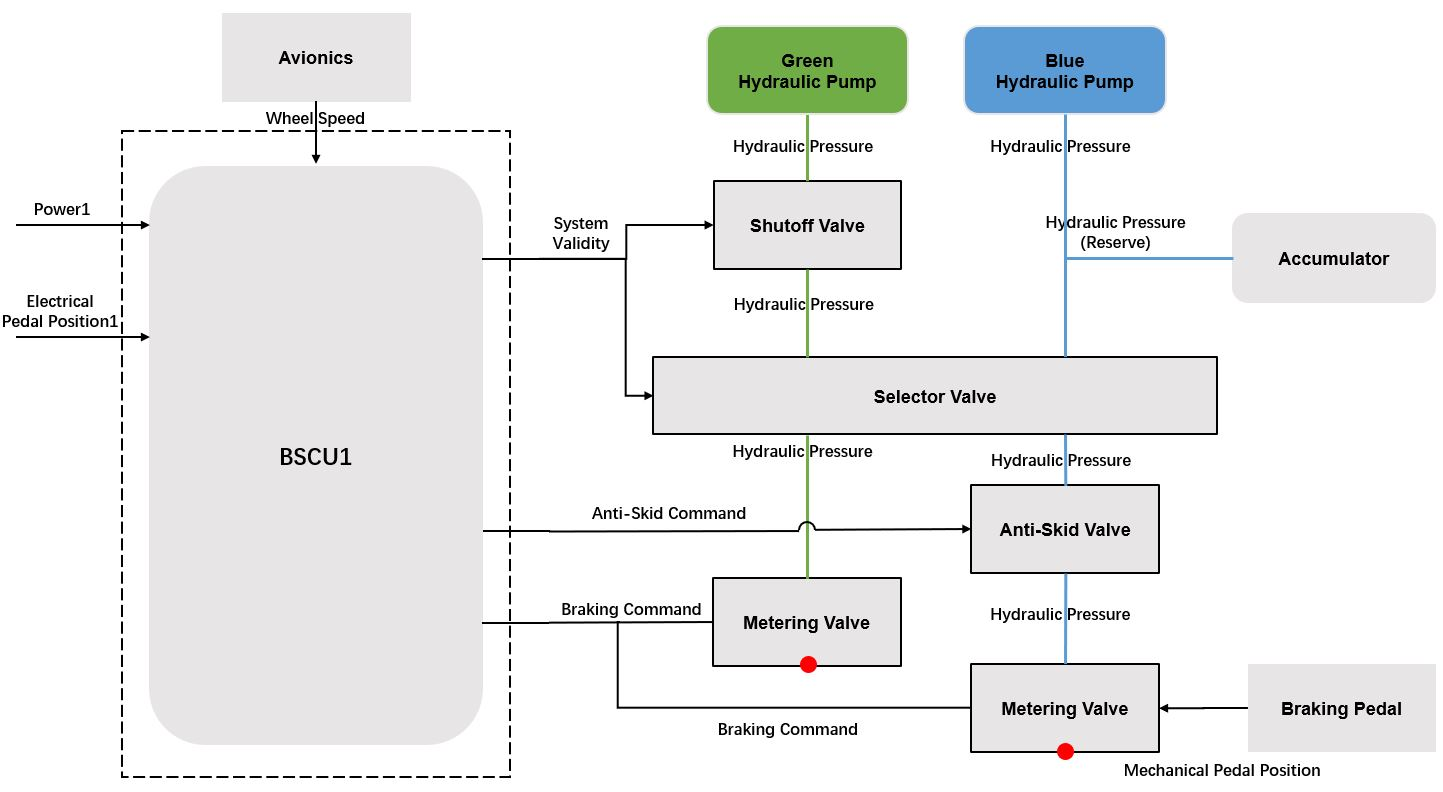
\includegraphics[width=85mm]{figure/Nominal.JPG}}
	\caption{The WBS BIP model of the nominal behavior}
	\label{WBS_BIP_Nominal}
\end{figure}

Figure 1 shows the WBS BIP model of the nominal behavior. The WBS is composed of an electronic control system and a physical system. The majority of the electronic control system is Braking System Control Unit(BSCU). The WBS receives several signals including the brake pedal position from upper level avionics system and electically forwards them to the BSCU. The BSCU also receives two power inputs from two independent power supply resources. As the result of computation, the BSCU in turn produces the system validity command, anti-skid command and braking command to the physical system. The physical system includes two hydraulic pressure lines which are supplied by the green/blue hydraulic pump respectively.

\emph{Operation Mode.} There are three operation modes for physical system. In \emph{normal mode}, the wheel brake is supported by the main hydraulic circuit, refers to the green hydraulic circuit. In \emph{alternate mode}, the wheel brake is supported by a second hydraulic circuit. This mode is standby and is selected automatically when the normal system fails. An accumulator supplies the \emph{emergency mode} when blue hydraulic supply is lost and the normal mode is not available.

\emph{Braking System Control Unit(BSCU).} According to the AIR6110 standard, for redundancy, the BSCU is composed of two independent channels, each channel has its own power supply and avioncs system inputs. Each channel has a command subsystem and a monitor subsystem. The monitor system generates the system validity command and the command system cauculates the anti-skid command and braking command. The BSCU will make an ultimate judgement call between each command output by the two channels respectively.

\emph{Hydraulic Pump.} In nominal system behavior, both the green and blue hydraulic pumps provide enough hydraulic pressure for their green/blue hydraulic circuit respectively. An accumulator is also a hydraulic pump to provide an emergency reserve of hydraulic pressure for blue hydraulic circuit in emergency mode.

\emph{Shutoff Valve.} The shutoff valve responds the system validity command from BSCU to decide whether to apply the hydraulic pressure to the selector valve in green hydraulic circuit or not. The system validity command is modeled in BIP as a boolean value.

\emph{Selector Valve.} The selector valve control the switch between green and blue hydraulic circuits mechanically. It outputs appropriate pressure from green hydraulic pump, and switches to blue hydraulic circuit as soon as it detects a lack of pressure in the green hydraulic circuit. In BIP model, the component selector valve 
only outputs pressure from either the green hydraulic circuit input or blue hydraulic circuit input at a time.

\emph{Anti-Skid Valve.} The anti-skid valve follows anti-skid command to control hydraulic pressure to the metering valve. It is used to restrict the hydraulic pressure to the wheel brake in order to prevent locking of the wheel. Wheel skid happens when the wheel is locked but the vehicle keeps a relative slid speed to the ground. We consider a loss of anti-skid function as a fault and will integrate it into nominal BIP model.

\emph{Metering Valve.} Metering valve, or metering servo valve controls pressure to the demanded level and provides regulation for the anti-skid function.

\section{Integrating Fault Trees Into WBS BIP model}
Before you begin to format your paper, first write and save the content as a 
separate text file. Complete all content and organizational editing before 
formatting. Please note sections \ref{AA}--\ref{SCM} below for more information on 
proofreading, spelling and grammar.

Keep your text and graphic files separate until after the text has been 
formatted and styled. Do not number text heads---{\LaTeX} will do that 
for you.

\subsection{Abbreviations and Acronyms}\label{AA}
Define abbreviations and acronyms the first time they are used in the text, 
even after they have been defined in the abstract. Abbreviations such as 
IEEE, SI, MKS, CGS, ac, dc, and rms do not have to be defined. Do not use 
abbreviations in the title or heads unless they are unavoidable.

\subsection{Units}
\begin{itemize}
\item Use either SI (MKS) or CGS as primary units. (SI units are encouraged.) English units may be used as secondary units (in parentheses). An exception would be the use of English units as identifiers in trade, such as ``3.5-inch disk drive''.
\item Avoid combining SI and CGS units, such as current in amperes and magnetic field in oersteds. This often leads to confusion because equations do not balance dimensionally. If you must use mixed units, clearly state the units for each quantity that you use in an equation.
\item Do not mix complete spellings and abbreviations of units: ``Wb/m\textsuperscript{2}'' or ``webers per square meter'', not ``webers/m\textsuperscript{2}''. Spell out units when they appear in text: ``. . . a few henries'', not ``. . . a few H''.
\item Use a zero before decimal points: ``0.25'', not ``.25''. Use ``cm\textsuperscript{3}'', not ``cc''.)
\end{itemize}

\subsection{Equations}
Number equations consecutively. To make your 
equations more compact, you may use the solidus (~/~), the exp function, or 
appropriate exponents. Italicize Roman symbols for quantities and variables, 
but not Greek symbols. Use a long dash rather than a hyphen for a minus 
sign. Punctuate equations with commas or periods when they are part of a 
sentence, as in:
\begin{equation}
a+b=\gamma\label{eq}
\end{equation}

Be sure that the 
symbols in your equation have been defined before or immediately following 
the equation. Use ``\eqref{eq}'', not ``Eq.~\eqref{eq}'' or ``equation \eqref{eq}'', except at 
the beginning of a sentence: ``Equation \eqref{eq} is . . .''

\subsection{\LaTeX-Specific Advice}

Please use ``soft'' (e.g., \verb|\eqref{Eq}|) cross references instead
of ``hard'' references (e.g., \verb|(1)|). That will make it possible
to combine sections, add equations, or change the order of figures or
citations without having to go through the file line by line.

Please don't use the \verb|{eqnarray}| equation environment. Use
\verb|{align}| or \verb|{IEEEeqnarray}| instead. The \verb|{eqnarray}|
environment leaves unsightly spaces around relation symbols.

Please note that the \verb|{subequations}| environment in {\LaTeX}
will increment the main equation counter even when there are no
equation numbers displayed. If you forget that, you might write an
article in which the equation numbers skip from (17) to (20), causing
the copy editors to wonder if you've discovered a new method of
counting.

{\BibTeX} does not work by magic. It doesn't get the bibliographic
data from thin air but from .bib files. If you use {\BibTeX} to produce a
bibliography you must send the .bib files. 

{\LaTeX} can't read your mind. If you assign the same label to a
subsubsection and a table, you might find that Table I has been cross
referenced as Table IV-B3. 

{\LaTeX} does not have precognitive abilities. If you put a
\verb|\label| command before the command that updates the counter it's
supposed to be using, the label will pick up the last counter to be
cross referenced instead. In particular, a \verb|\label| command
should not go before the caption of a figure or a table.

Do not use \verb|\nonumber| inside the \verb|{array}| environment. It
will not stop equation numbers inside \verb|{array}| (there won't be
any anyway) and it might stop a wanted equation number in the
surrounding equation.

\subsection{Some Common Mistakes}\label{SCM}
\begin{itemize}
\item The word ``data'' is plural, not singular.
\item The subscript for the permeability of vacuum $\mu_{0}$, and other common scientific constants, is zero with subscript formatting, not a lowercase letter ``o''.
\item In American English, commas, semicolons, periods, question and exclamation marks are located within quotation marks only when a complete thought or name is cited, such as a title or full quotation. When quotation marks are used, instead of a bold or italic typeface, to highlight a word or phrase, punctuation should appear outside of the quotation marks. A parenthetical phrase or statement at the end of a sentence is punctuated outside of the closing parenthesis (like this). (A parenthetical sentence is punctuated within the parentheses.)
\item A graph within a graph is an ``inset'', not an ``insert''. The word alternatively is preferred to the word ``alternately'' (unless you really mean something that alternates).
\item Do not use the word ``essentially'' to mean ``approximately'' or ``effectively''.
\item In your paper title, if the words ``that uses'' can accurately replace the word ``using'', capitalize the ``u''; if not, keep using lower-cased.
\item Be aware of the different meanings of the homophones ``affect'' and ``effect'', ``complement'' and ``compliment'', ``discreet'' and ``discrete'', ``principal'' and ``principle''.
\item Do not confuse ``imply'' and ``infer''.
\item The prefix ``non'' is not a word; it should be joined to the word it modifies, usually without a hyphen.
\item There is no period after the ``et'' in the Latin abbreviation ``et al.''.
\item The abbreviation ``i.e.'' means ``that is'', and the abbreviation ``e.g.'' means ``for example''.
\end{itemize}
An excellent style manual for science writers is \cite{b7}.

\subsection{Authors and Affiliations}
\textbf{The class file is designed for, but not limited to, six authors.} A 
minimum of one author is required for all conference articles. Author names 
should be listed starting from left to right and then moving down to the 
next line. This is the author sequence that will be used in future citations 
and by indexing services. Names should not be listed in columns nor group by 
affiliation. Please keep your affiliations as succinct as possible (for 
example, do not differentiate among departments of the same organization).

\subsection{Identify the Headings}
Headings, or heads, are organizational devices that guide the reader through 
your paper. There are two types: component heads and text heads.

Component heads identify the different components of your paper and are not 
topically subordinate to each other. Examples include Acknowledgments and 
References and, for these, the correct style to use is ``Heading 5''. Use 
``figure caption'' for your Figure captions, and ``table head'' for your 
table title. Run-in heads, such as ``Abstract'', will require you to apply a 
style (in this case, italic) in addition to the style provided by the drop 
down menu to differentiate the head from the text.

Text heads organize the topics on a relational, hierarchical basis. For 
example, the paper title is the primary text head because all subsequent 
material relates and elaborates on this one topic. If there are two or more 
sub-topics, the next level head (uppercase Roman numerals) should be used 
and, conversely, if there are not at least two sub-topics, then no subheads 
should be introduced.

\subsection{Figures and Tables}
\paragraph{Positioning Figures and Tables} Place figures and tables at the top and 
bottom of columns. Avoid placing them in the middle of columns. Large 
figures and tables may span across both columns. Figure captions should be 
below the figures; table heads should appear above the tables. Insert 
figures and tables after they are cited in the text. Use the abbreviation 
``Fig.~\ref{fig}'', even at the beginning of a sentence.

\begin{table}[htbp]
\caption{Table Type Styles}
\begin{center}
\begin{tabular}{|c|c|c|c|}
\hline
\textbf{Table}&\multicolumn{3}{|c|}{\textbf{Table Column Head}} \\
\cline{2-4} 
\textbf{Head} & \textbf{\textit{Table column subhead}}& \textbf{\textit{Subhead}}& \textbf{\textit{Subhead}} \\
\hline
copy& More table copy$^{\mathrm{a}}$& &  \\
\hline
\multicolumn{4}{l}{$^{\mathrm{a}}$Sample of a Table footnote.}
\end{tabular}
\label{tab1}
\end{center}
\end{table}

\begin{figure}[htbp]
\centerline{
\includegraphics{figure/fig1.png}}
\caption{Example of a figure caption.}
\label{fig}
\end{figure}

Figure Labels: Use 8 point Times New Roman for Figure labels. Use words 
rather than symbols or abbreviations when writing Figure axis labels to 
avoid confusing the reader. As an example, write the quantity 
``Magnetization'', or ``Magnetization, M'', not just ``M''. If including 
units in the label, present them within parentheses. Do not label axes only 
with units. In the example, write ``Magnetization (A/m)'' or ``Magnetization 
\{A[m(1)]\}'', not just ``A/m''. Do not label axes with a ratio of 
quantities and units. For example, write ``Temperature (K)'', not 
``Temperature/K''.

\section{Verification Methodology and Experiments}

\section*{Acknowledgment}

The preferred spelling of the word ``acknowledgment'' in America is without 
an ``e'' after the ``g''. Avoid the stilted expression ``one of us (R. B. 
G.) thanks $\ldots$''. Instead, try ``R. B. G. thanks$\ldots$''. Put sponsor 
acknowledgments in the unnumbered footnote on the first page.

\section*{References}

Please number citations consecutively within brackets \cite{b1}. The 
sentence punctuation follows the bracket \cite{b2}. Refer simply to the reference 
number, as in \cite{b3}---do not use ``Ref. \cite{b3}'' or ``reference \cite{b3}'' except at 
the beginning of a sentence: ``Reference \cite{b3} was the first $\ldots$''

Number footnotes separately in superscripts. Place the actual footnote at 
the bottom of the column in which it was cited. Do not put footnotes in the 
abstract or reference list. Use letters for table footnotes.

Unless there are six authors or more give all authors' names; do not use 
``et al.''. Papers that have not been published, even if they have been 
submitted for publication, should be cited as ``unpublished'' \cite{b4}. Papers 
that have been accepted for publication should be cited as ``in press'' \cite{b5}. 
Capitalize only the first word in a paper title, except for proper nouns and 
element symbols.

For papers published in translation journals, please give the English 
citation first, followed by the original foreign-language citation \cite{b6}.

\begin{thebibliography}{00}
\bibitem{b1} G. Eason, B. Noble, and I. N. Sneddon, ``On certain integrals of Lipschitz-Hankel type involving products of Bessel functions,'' Phil. Trans. Roy. Soc. London, vol. A247, pp. 529--551, April 1955.
\bibitem{b2} J. Clerk Maxwell, A Treatise on Electricity and Magnetism, 3rd ed., vol. 2. Oxford: Clarendon, 1892, pp.68--73.
\bibitem{b3} I. S. Jacobs and C. P. Bean, ``Fine particles, thin films and exchange anisotropy,'' in Magnetism, vol. III, G. T. Rado and H. Suhl, Eds. New York: Academic, 1963, pp. 271--350.
\bibitem{b4} K. Elissa, ``Title of paper if known,'' unpublished.
\bibitem{b5} R. Nicole, ``Title of paper with only first word capitalized,'' J. Name Stand. Abbrev., in press.
\bibitem{b6} Y. Yorozu, M. Hirano, K. Oka, and Y. Tagawa, ``Electron spectroscopy studies on magneto-optical media and plastic substrate interface,'' IEEE Transl. J. Magn. Japan, vol. 2, pp. 740--741, August 1987 [Digests 9th Annual Conf. Magnetics Japan, p. 301, 1982].
\bibitem{b7} M. Young, The Technical Writer's Handbook. Mill Valley, CA: University Science, 1989.
\end{thebibliography}

\end{document}
